% fig_triptime.tex
% Operate time vs Rf for fixed and adaptive TMS
% Values from hif_sim.py (inception=0deg, loading=0.8pu)
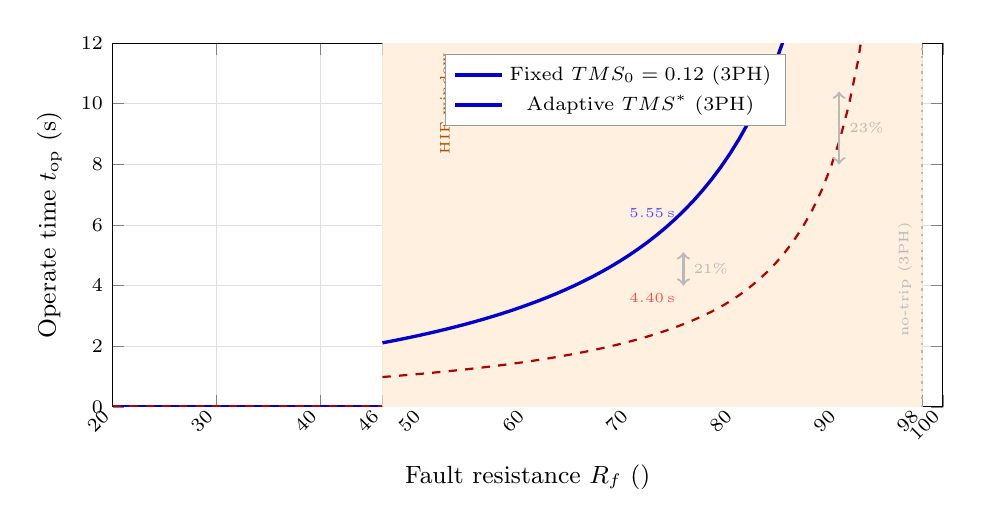
\begin{tikzpicture}
\begin{axis}[
  width=\columnwidth, height=6.2cm,
  xlabel={Fault resistance $R_f$ (\si{\ohm})},
  ylabel={Operate time $t_{\mathrm{op}}$ (s)},
  xmin=20, xmax=100,
  ymin=0, ymax=12,
  xtick={20,30,40,46,50,60,70,80,90,98,100},
  xticklabel style={rotate=45,anchor=east},
  ytick={0,2,4,6,8,10,12},
  grid=both,
  grid style={gray!25,line width=0.3pt},
  tick label style={font=\scriptsize},
  label style={font=\small},
  legend style={at={(0.40,0.97)},anchor=north west,
                font=\scriptsize,fill=white,draw=black!40},
  clip=true]

  % HIF window
  \addplot[fill=orange!12,draw=none,forget plot]
    coordinates {(46,0)(98,0)(98,12)(46,12)} \closedcycle;
  \node[font=\tiny,orange!65!black,rotate=90]
    at (axis cs:52,10) {HIF window};

  % ---- Analytical curve: fixed TMS = 0.12, 3PH ----
  % t = 0.12*13.5 / (M-1), M=0.884/sqrt((0.02+Rf/121)^2+0.09)
  \addplot[blue!80!black,very thick,samples=60,domain=46:98]
    { 0.12 * 13.5 / ( 0.884/sqrt((0.02+x/121)^2+0.09) - 1.0 ) };
  \addplot[blue!80!black,very thick,domain=20:46]
    coordinates {(20,0.02)(46,0.02)};
  \addlegendentry{Fixed $TMS_0=0.12$ (3PH)}

  % ---- Analytical curve: adaptive TMS, 3PH ----
  % Iss = 1/(1.95+Rf/121), fHIF = clip(Iss/0.51,0.3,1), Keff=0.08 (HIF zone)
  % TMS* = clip(0.08*0.83*fHIF, 0.05, 0.25)
  \addplot[red!70!black,thick,dashed,samples=60,domain=46:98]
    { 13.5 * max(0.08*0.83*min(max((1/(1.95+x/121))/0.51,0.3),1.0),0.05)
      / ( 0.884/sqrt((0.02+x/121)^2+0.09) - 1.0 ) };
  \addplot[red!70!black,thick,dashed,domain=20:46]
    coordinates {(20,0.02)(46,0.02)};
  \addlegendentry{Adaptive $TMS^*$ (3PH)}

  % No-trip boundary
  \draw[gray!55,thick,dotted]
    (axis cs:98,0) -- (axis cs:98,12)
    node[above,rotate=90,font=\tiny,gray!55,pos=0.35]
    {no-trip (3PH)};

  % Improvement markers (from hif_sim.py)
  \draw[<->,gray!55,thick]
    (axis cs:75,4.0) -- (axis cs:75,5.1)
    node[midway,right,font=\tiny,gray!55]{21\%};
  \draw[<->,gray!55,thick]
    (axis cs:90,8.0) -- (axis cs:90,10.4)
    node[midway,right,font=\tiny,gray!55]{23\%};

  % Simulation result markers
  \node[font=\tiny\bfseries,blue!70,align=center]
    at (axis cs:72,6.4) {$5.55\,\mathrm{s}$};
  \node[font=\tiny\bfseries,red!70,align=center]
    at (axis cs:72,3.6) {$4.40\,\mathrm{s}$};

\end{axis}
\end{tikzpicture}
